\documentclass[aspectratio=169,10pt]{beamer}
\usepackage{../common/beamer_theme_bio}

\title{\textbf{Biostatistiques Appliquées}}
\subtitle{Chapitre IV : Régression Non Linéaire en Biochimie \& Modélisation Cinétique}
\author{\textbf{Dr. Sarra BENMOUMOU (Ph.D.)}}
\institute{
  Faculté des Sciences --- Département de Biologie\\
  Master 2 : Biochimie Appliquée\\
  \textbf{Université M'Hamed Bougara de Boumerdès (UMBB)}
}
\date{Année Universitaire 2024 -- 2025}

\begin{document}

\begin{frame}[plain]
  \titlepage
\end{frame}

\begin{frame}{Plan Détaillé du Chapitre IV}
  \tableofcontents
\end{frame}

% ========================================================
\section{Pourquoi la Régression Non Linéaire ?}
% ========================================================

\begin{frame}{L'Erreur Historique des Linéarisations Graphiques}
  \begin{columns}[onlytextwidth, T]
    \begin{column}{0.48\linewidth}
      \begin{warnbox}{Le Piège de Lineweaver-Burk ($1/v = f(1/[S])$)}
        Autrefois indispensable avant l'informatique pour tracer à la règle :
        \begin{itemize}
          \item Prend l'inverse des mesures ($1/v$).
          \item Déforme dramatiquement la distribution de l'erreur expérimentale (qui n'est plus normale).
          \item Donne un poids statistique démesuré aux mesures les plus imprécises (très faibles vitesses à très faible $[S]$).
        \end{itemize}
      \end{warnbox}
    \end{column}
    \begin{column}{0.48\linewidth}
      \begin{conceptbox}{Le Standard Moderne : L'Ajustement NLLS Direct}
        Ajuster directement l'équation hyperbolique sur les données brutes :
        \begin{equation*}
          \min_{V_{\max}, K_m} \sum_{i=1}^n \left( v_i - \frac{V_{\max} [S]_i}{K_m + [S]_i} \right)^2
        \end{equation*}
        \textbf{Algorithme standard :} \textbf{Levenberg-Marquardt} (itératif, préserve l'homoscédasticité des mesures réelles).
      \end{conceptbox}
    \end{column}
  \end{columns}
\end{frame}

\begin{frame}{Démonstration Expérimentale : NLLS Direct vs. Lineweaver-Burk}
  \begin{center}
    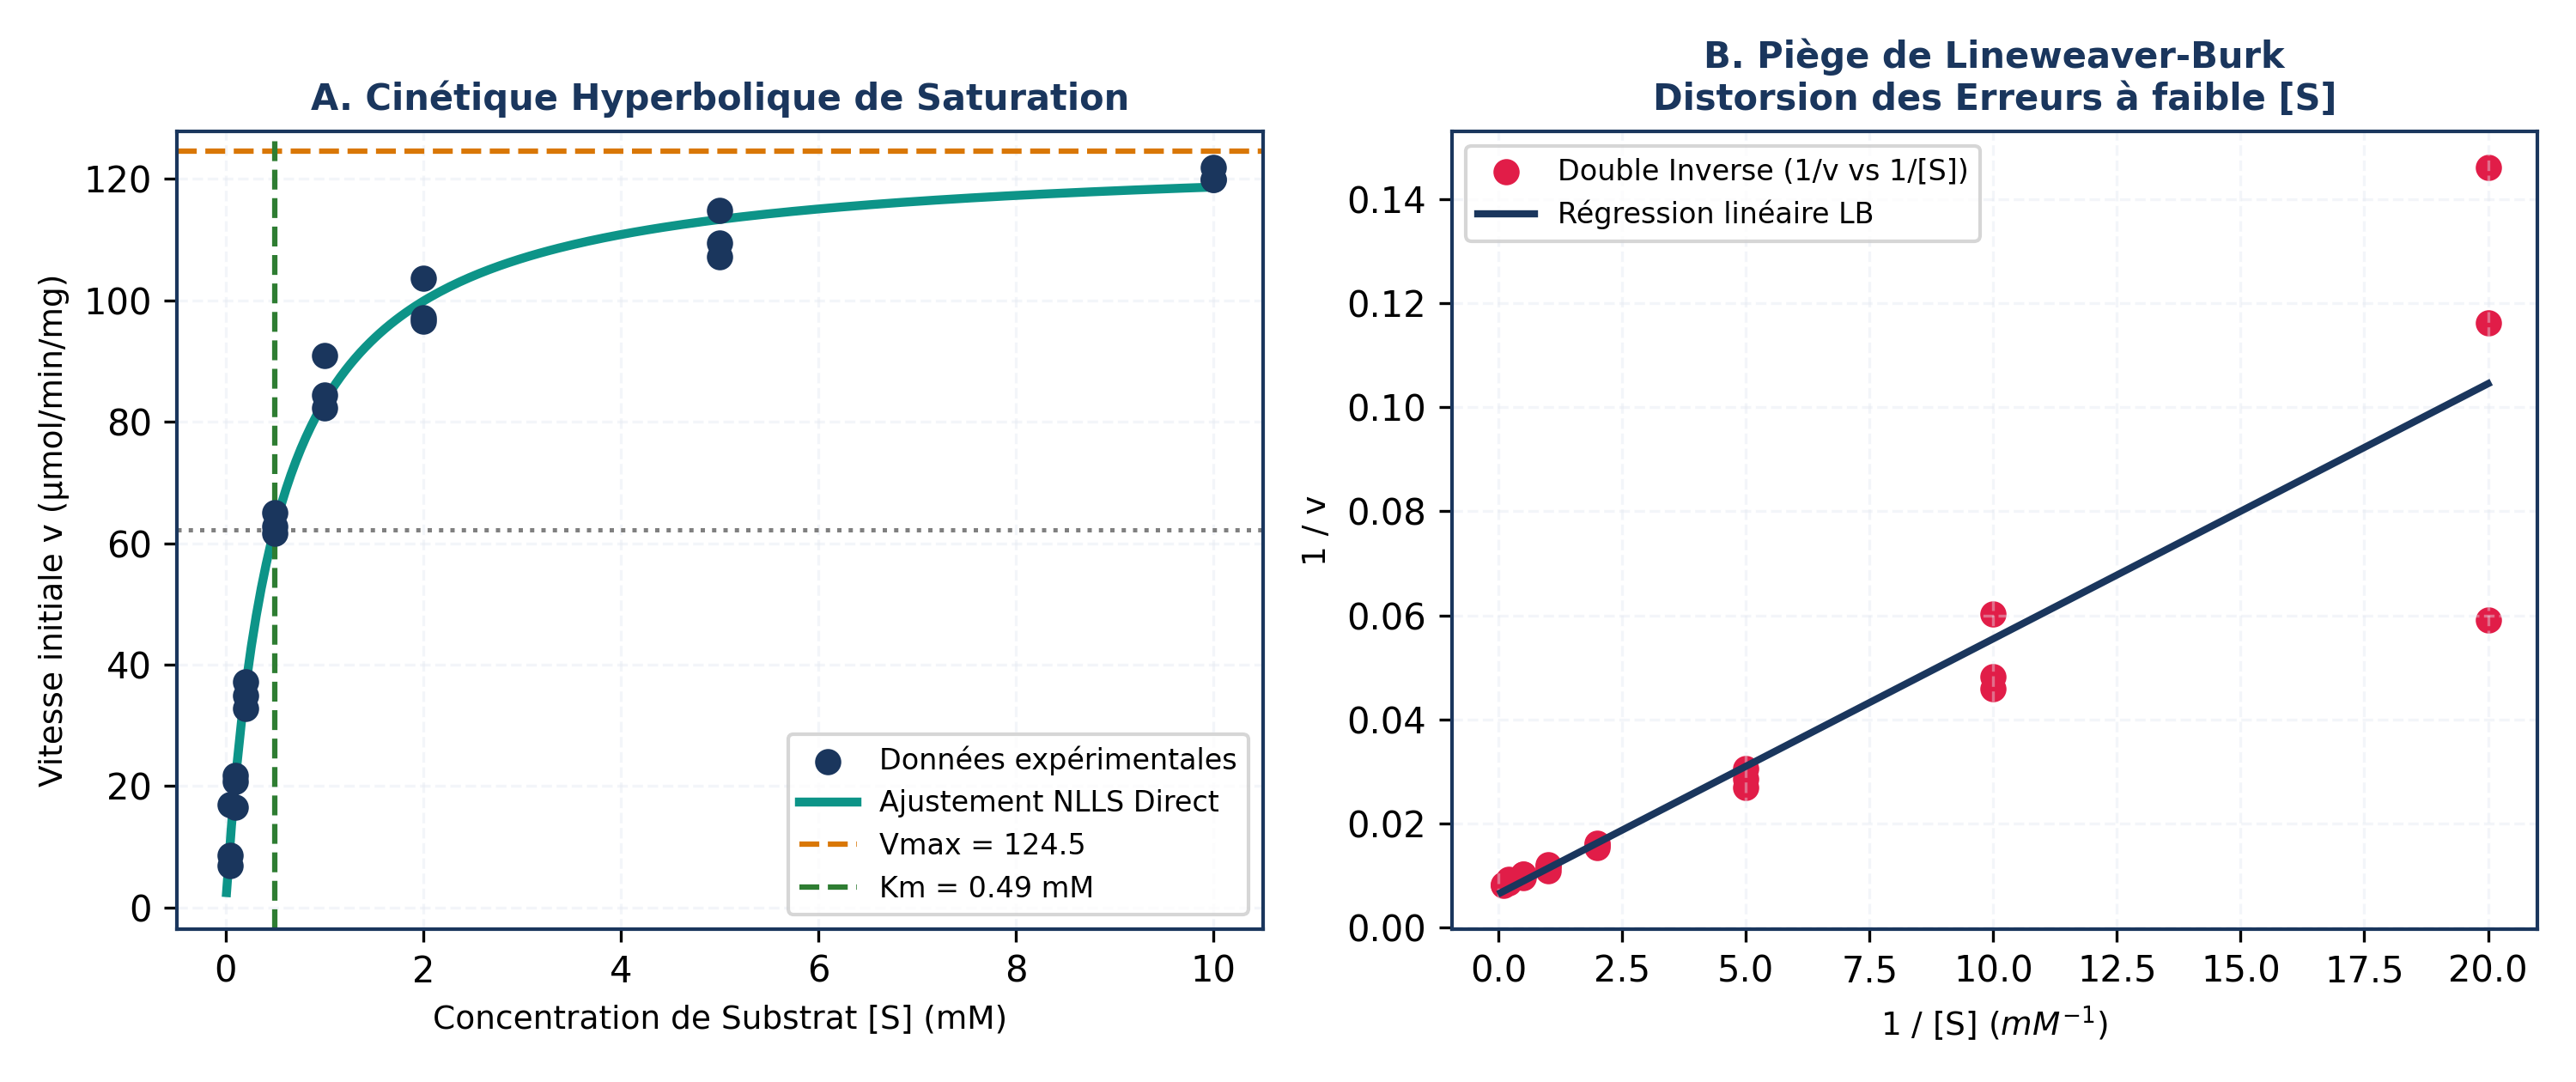
\includegraphics[width=0.90\linewidth]{../figures/fig04_nlls_vs_lineweaver_burk.png}
  \end{center}
  \vspace{-2mm}
  \begin{columns}[onlytextwidth, T]
    \begin{column}{0.48\linewidth}
      {\footnotesize \textbf{À gauche (NLLS Direct) :} Courbe hyperbolique ajustée sur les points expérimentaux avec estimation robuste de $V_{\max}$ et $K_m$.}
    \end{column}
    \begin{column}{0.48\linewidth}
      {\footnotesize \textbf{À droite (Lineweaver-Burk) :} Les points à faible concentration s'envolent à droite et faussent la pente de 35\% !}
    \end{column}
  \end{columns}
\end{frame}

% ========================================================
\section{Modèles de Saturation \& Allostérie}
% ========================================================

\begin{frame}{Modèle de Monod / Michaelis-Menten \& Coopérativité de Hill}
  \begin{columns}[onlytextwidth, T]
    \begin{column}{0.48\linewidth}
      \begin{conceptbox}{1. Michaelis-Menten (Hyperbolique)}
        \begin{equation*}
          v = \frac{V_{\max} \cdot [S]}{K_m + [S]}
        \end{equation*}
        \begin{itemize}
          \item \textbf{$V_{\max}$ :} Capacité catalytique maximale quand tous les sites actifs sont saturés.
          \item \textbf{$K_m$ :} Concentration en substrat pour laquelle $v = V_{\max} / 2$ (reflète l'affinité apparente).
        \end{itemize}
      \end{conceptbox}
    \end{column}
    \begin{column}{0.48\linewidth}
      \begin{conceptbox}{2. Équation de Hill (Enzymes Allostériques)}
        \begin{equation*}
          v = \frac{V_{\max} \cdot [S]^h}{K_{0.5}^h + [S]^h}
        \end{equation*}
        \begin{itemize}
          \item \textbf{$h > 1$ :} Coopérativité positive (courbe sigmoïde, ex : Hémoglobine, Phosphofructokinase).
          \item \textbf{$h < 1$ :} Coopérativité négative.
          \item \textbf{$h = 1$ :} Retour au modèle classique de Michaelis-Menten.
        \end{itemize}
      \end{conceptbox}
    \end{column}
  \end{columns}
\end{frame}

% ========================================================
\section{Modèles Sigmoïdes (4PL) \& Exponentiels}
% ========================================================

\begin{frame}{Le Modèle Sigmoïde à 4 Paramètres (4PL) pour l'ELISA}
  \begin{center}
    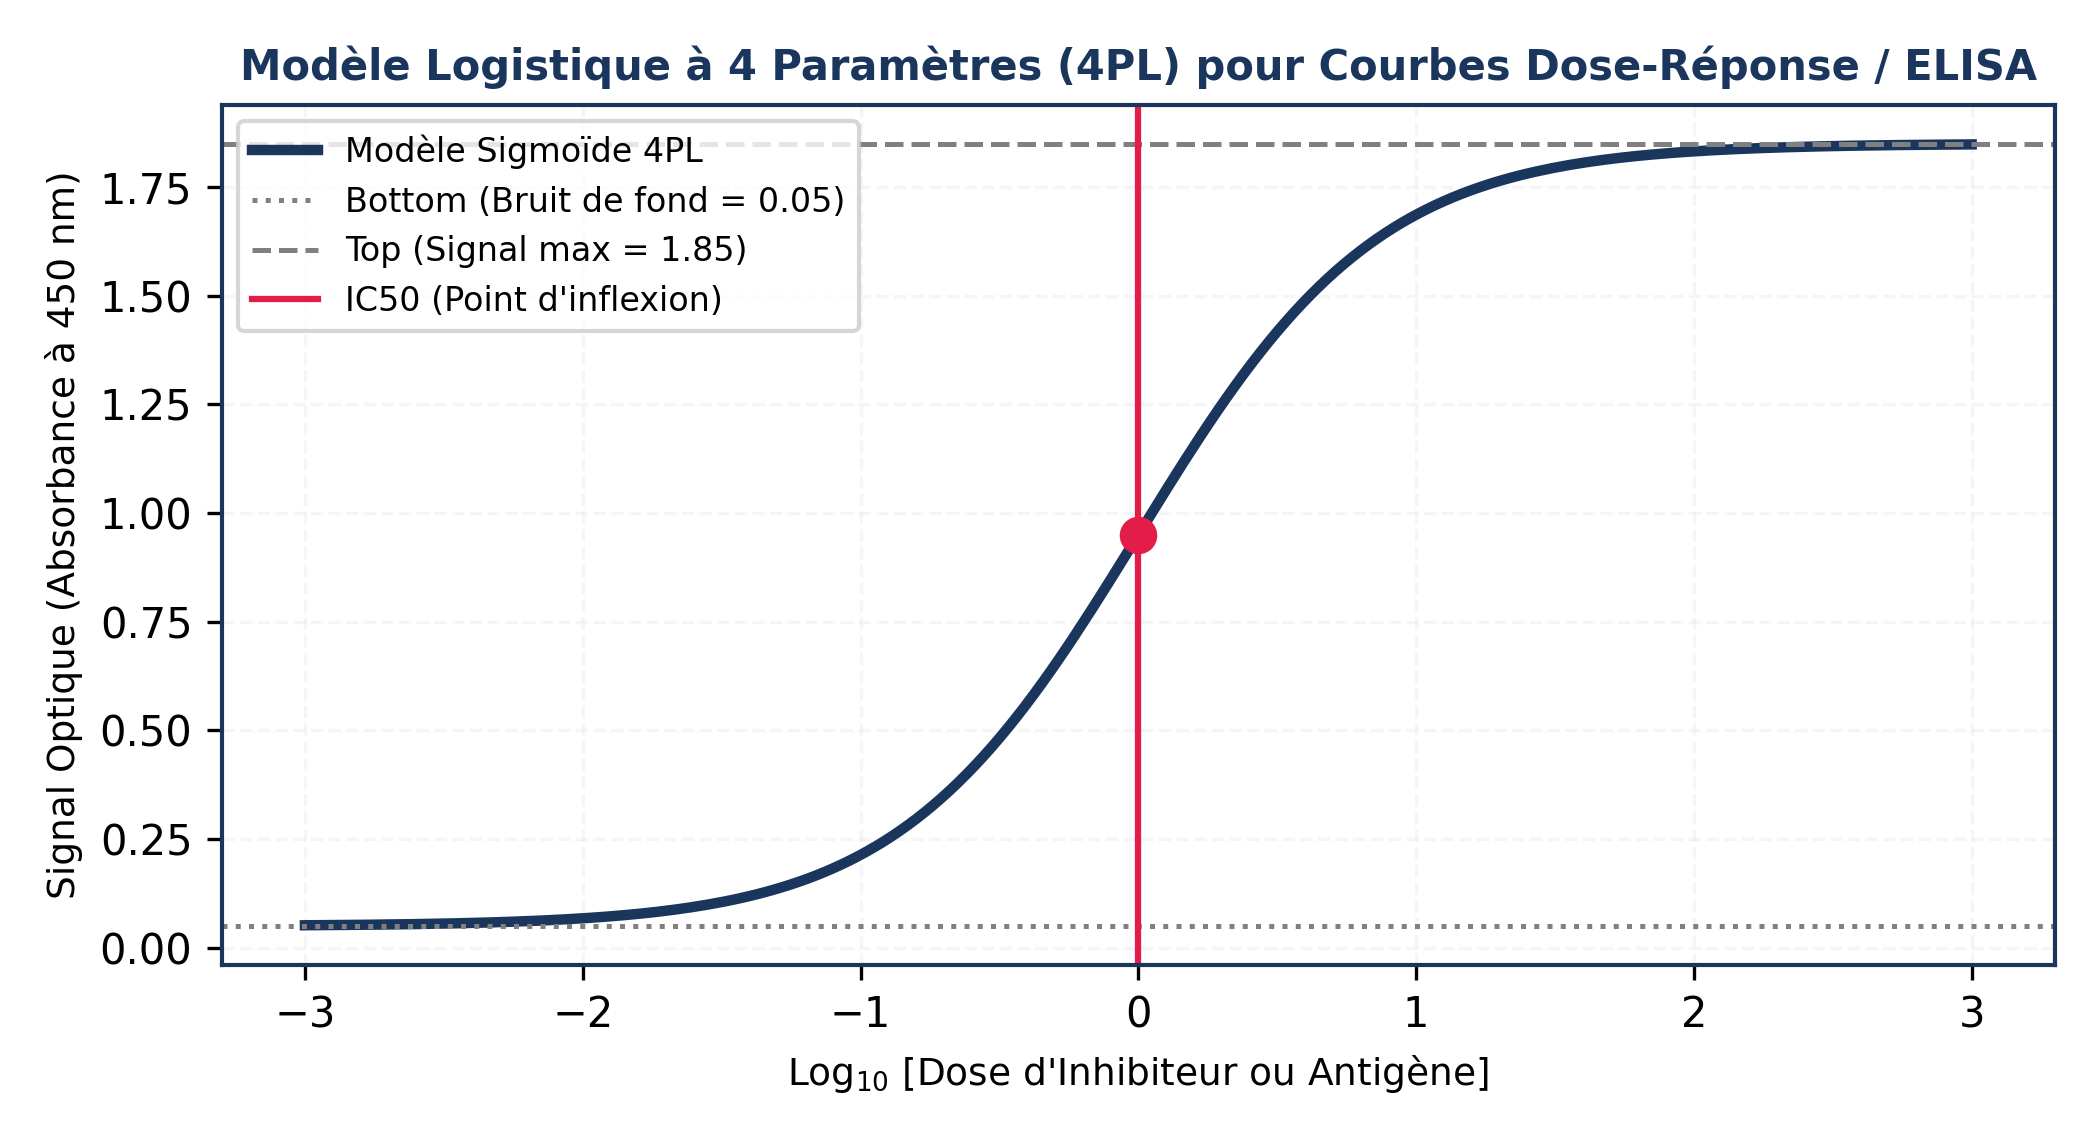
\includegraphics[width=0.85\linewidth]{../figures/fig04_sigmoidal_4pl_elisa.png}
  \end{center}
  \vspace{-2mm}
  \begin{conceptbox}{Équation du Modèle 4PL (Pharmacologie \& Immunologie)}
    $$Y = \text{Bottom} + \frac{\text{Top} - \text{Bottom}}{1 + 10^{(\log IC_{50} - X) \cdot \text{HillSlope}}}$$
    \begin{itemize}
      \item \textbf{Bottom / Top :} Paliers d'absorbance minimale (bruit) et maximale (saturation des anticorps).
      \item \textbf{$IC_{50}$ / $EC_{50}$ :} Concentration médiane d'inhibition ou d'effet au point d'inflexion.
    \end{itemize}
  \end{conceptbox}
\end{frame}

\begin{frame}{Modèles Exponentiels, Bêta \& Gamma}
  \begin{columns}[onlytextwidth, T]
    \begin{column}{0.48\linewidth}
      \textbf{\color{BioNavy}1. Modèles Exponentiels}
      \begin{itemize}
        \item \textbf{Croissance bactérienne :} $N(t) = N_0 e^{\mu t}$ (temps de doublement $t_d = \frac{\ln 2}{\mu}$).
        \item \textbf{Pharmacocinétique d'élimination :} $C(t) = C_0 e^{-k_e t}$ (demi-vie $t_{1/2} = \frac{\ln 2}{k_e}$).
      \end{itemize}
    \end{column}
    \begin{column}{0.48\linewidth}
      \textbf{\color{BioTeal}2. Modèles Bêta \& Gamma}
      \begin{itemize}
        \item \textbf{Modèle Gamma :} Modélise des cinétiques enzymatiques avec phase de latence (lag-phase) ou des temps de survie cellulaire asymétriques.
        \item \textbf{Modèle Bêta :} Très adapté aux courbes d'activité enzymatique en cloche asymétrique en fonction du pH ou de la température.
      \end{itemize}
    \end{column}
  \end{columns}
\end{frame}

\begin{frame}[plain]
  \begin{center}
    \vspace{1.8cm}
    {\Huge\color{BioNavy}\textbf{Fin du Chapitre IV}}\\[0.8cm]
    {\large Prochaine étape : L'Analyse en Composantes Principales (ACP)}\\[1.2cm]
    \textbf{Dr. Sarra BENMOUMOU (Ph.D.)}\\
    \small Faculté des Sciences --- Département de Biologie\\
    \textbf{Université M'Hamed Bougara de Boumerdès (UMBB)}
  \end{center}
\end{frame}

\end{document}
